\documentclass[10pt, landscape]{article}
\usepackage[scaled=0.92]{helvet}
\usepackage{calc}
\usepackage{multicol}
\usepackage{ifthen}
\usepackage[a4paper,margin=3mm,landscape]{geometry}
\usepackage{amsmath,amsthm,amsfonts,amssymb}
\usepackage{color,graphicx,overpic}
\usepackage{hyperref}
\usepackage{newtxtext} 
\usepackage{enumitem}
\usepackage{amssymb}
\usepackage[table]{xcolor}
\usepackage{vwcol}
\usepackage{tikz}
\usetikzlibrary{arrows.meta}
\usetikzlibrary{calc}
\usepackage{mathtools}
\usepackage{nicematrix}
%For pictures / figures
\usepackage{color,graphicx,overpic}
\graphicspath{ {./images/} }
% for relations
\usepackage{cancel}
\usepackage{ mathrsfs }
\graphicspath{ {./images/} }
\setlist{nosep}


\pdfinfo{
  /Title (CG1111A-Quiz2.pdf)
  /Creator (TeX)
  /Producer (pdfTeX 1.40.0)
  /Author (Seamus)
  /Subject (Example)
  /Keywords (pdflatex, latex,pdftex,tex)}

% Turn off header and footer
\pagestyle{empty}

\newenvironment{tightcenter}{%
  \setlength\topsep{0pt}
  \setlength\parskip{0pt}
  \begin{center}
}{%
  \end{center}
}

% redefine section commands to use less space
\makeatletter
\renewcommand{\section}{\@startsection{section}{1}{0mm}%
                                {-1ex plus -.5ex minus -.2ex}%
                                {0.5ex plus .2ex}%x
                                {\normalfont\large\bfseries}}
\renewcommand{\subsection}{\@startsection{subsection}{2}{0mm}%
                                {-1explus -.5ex minus -.2ex}%
                                {0.5ex plus .2ex}%
                                {\normalfont\normalsize\bfseries}}
\renewcommand{\subsubsection}{\@startsection{subsubsection}{3}{0mm}%
                                {-1ex plus -.5ex minus -.2ex}%
                                {1ex plus .2ex}%
                                {\normalfont\small\bfseries}}%
\renewcommand{\familydefault}{\sfdefault}
\renewcommand\rmdefault{\sfdefault}
% makes nested numbering (e.g. 1.1.1, 1.1.2, etc)
\renewcommand{\labelenumii}{\theenumii}
\renewcommand{\theenumii}{\theenumi.\arabic{enumii}.}
\renewcommand\labelitemii{•}
%  for logical not operator
\renewcommand{\lnot}{\mathord{\sim}}
\renewcommand{\bf}[1]{\textbf{#1}}
\newcommand{\abs}[1]{\vert #1 \vert}
\newcommand{\Mod}[1]{\ \mathrm{mod}\ #1}

\makeatother
\definecolor{myblue}{cmyk}{1,.72,0,.38}
\everymath\expandafter{\the\everymath \color{myblue}}
% Define BibTeX command
\def\BibTeX{{\rm B\kern-.05em{\sc i\kern-.025em b}\kern-.08em
    T\kern-.1667em\lower.7ex\hbox{E}\kern-.125emX}}
\let\iff\leftrightarrow
\let\Iff\Leftrightarrow
\let\then\rightarrow
\let\Then\Rightarrow

% Don't print section numbers
\setcounter{secnumdepth}{0}

\setlength{\parindent}{0pt}
\setlength{\parskip}{0pt plus 0.5ex}
%% this changes all items (enumerate and itemize)
\setlength{\leftmargini}{0.5cm}
\setlength{\leftmarginii}{0.5cm}
\setlist[itemize,1]{leftmargin=2mm,labelindent=1mm,labelsep=1mm}
\setlist[itemize,2]{leftmargin=4mm,labelindent=1mm,labelsep=1mm}

%My Environments
\newtheorem{example}[section]{Example}
% -----------------------------------------------------------------------

\begin{document}
\raggedright
\footnotesize
\begin{multicols}{4}


% multicol parameters
% These lengths are set only within the two main columns
\setlength{\columnseprule}{0.25pt}
\setlength{\premulticols}{1pt}
\setlength{\postmulticols}{1pt}
\setlength{\multicolsep}{1pt}
\setlength{\columnsep}{2pt}

\begin{center}
    \fbox{%
        \parbox{0.8\linewidth}{\centering \textcolor{black}{
            {\Large\textbf{CS2030S Midterm}}
            \\ \normalsize{AY24/25 sem 2}}
            \\ {\footnotesize \textcolor{myblue}{github.com/mendax1234}} 
        }%
    }
\end{center}

\section{Intro to OOP}
\begin{enumerate}
    \item \textbf{(Constructor}): If your class includes a \textbf{constructor with parameters}, you are required to \textbf{provide arguments} when creating an object using that constructor.
    \item \textbf{(Target)}: \texttt{object.method()}, \texttt{object} is the \textbf{target}.
    \item \textbf{(Initialization)}: Any \textit{reference} variable that is not initialized will have \textit{null}. Any \textit{primitive} type variable will have either 0 or false (boolean).
    \item \textbf{(Java)}: \textbf{Java} is a \textbf{statically typed} and \textbf{strongly typed} language.
    \begin{itemize}
        \item \textbf{Statically typed}: the variable can only hold values of the \textbf{declared type}. (Any subtype of the declared type is allowed).
        \item \textbf{Strongly typed}: Java compiler enforces a \textbf{stricter type checking rule to ensure type safety}. These rules include:
        \begin{itemize}
            \item \textbf{Valid subtype relationship when assigning one variable to another}: \textbf{Implicit narrowing conversion} is not allowed and \textbf{Type casting that makes no sense} is not allowed. (No subtype relationship).
        \end{itemize}
        \item \textbf{Floating point number} is treated as \texttt{double} by default. \textbf{Integer Literal} is treated as \texttt{int} by default.
        \item \textbf{Local variables won't be initialized} and accessing \textbf{uninitialized local variables} will generate \textbf{compile error}!
        \item \textbf{Subtype Relationship}
        \begin{itemize}
            \item \textbf{Primitive type}: \\
            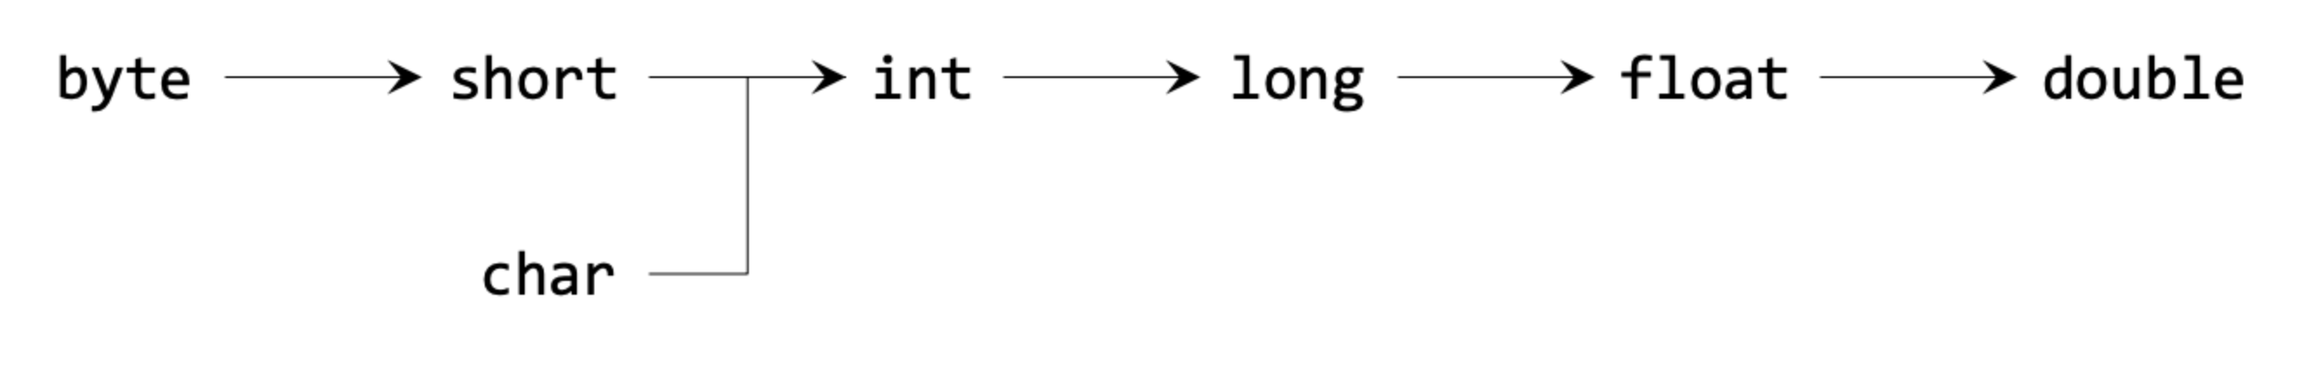
\includegraphics[width=1\linewidth]{Paper/Midterm/images/midterm-1.png}
            \item \textbf{Wrapper class}: \texttt{Number} is the \textbf{superclass} of \texttt{Integer, Double, BigInteger, Long} etc.
        \end{itemize}
        \item \textbf{We cannot instantiate one object twice}, e.g. calling \texttt{Circle c1 = new Circle();} twice will generate a \textbf{compile error}!
        \item We \textbf{cannot change the CTT of a variable}. So, if we have declared \texttt{Circle c}, we \textbf{cannot use} \texttt{String c} anymore in the same segment.
        \item Java is a \textbf{strongly typed language}, but it allows \textbf{widening type conversion} and will do this \textbf{automatically without explicit casting}.
        \item In Java, two types without a subtype relationship \textbf{cannot} be casted.
        \item \textbf{Nested method calling}: In Java, the nested method call is executed from \textbf{left to right}. e.g. \texttt{Box.of("string").map(new StringLength()).map(new AddOne());}, the left \texttt{.map} will be executed first.
        \item \textbf{method return}: Suppose the return type of a method is \textbf{T}, inside this method, you can actually return the \textbf{subtype} of \textbf{T}.
        \item \textbf{Reflexivity of subtype}: If \texttt{A<:B, B<:C}, then \texttt{A<:C}. Pay attention to the reflexivity!!! It may generate all the correct answers!
    \end{itemize}
    \item \textbf{Information Hiding}:
    \begin{itemize}
        \item \textbf{fields} should be declared as \texttt{private}
        \item \textbf{methods} should be declared as \texttt{public}
    \end{itemize}
\end{enumerate}

\section{More on OOP}
\begin{enumerate}
    \item \textbf{Modifier}
    \begin{itemize}
        \item \textbf{Access Modifier}: Private fields are accessible to all methods within the same class, regardless of which instance is being accessed.
        \item \textbf{Static field and methods}:
        \begin{itemize}
            \item A \textbf{static field} should be something that is \textbf{shared among all instances} of that class.
            \item A \textbf{static method} performs a task which \textbf{doesn’t need to access the data from any instance}.
            \item In \textbf{static methods}, we \textbf{cannot access any instance fields or call other instance methods}, the keyword \texttt{this} is also \textbf{not allowed}!
            \item \textbf{Static fields} can be \textbf{accessed} from \textbf{non-static methods.}
        \end{itemize}
        \item \textbf{\texttt{final}}: 
        \begin{itemize}
            \item \texttt{final} in a \textbf{field declaration} prevents \textbf{re-assignment}, in a \textbf{class declaration} prevents \textbf{inheritance}, in a \textbf{method declaration} prevents \textbf{overriding}.
        \end{itemize}
        \item \textbf{Modifier Order}: an example is \texttt{public static final void}, this is to declare a \textbf{constant}
    \end{itemize}
    \item \textbf{Heap and Stack}
    \begin{itemize}
        \item \textbf{Stack}: The stack is where all variables (\textbf{primitive types and object references}) are stored. The stack contains \textbf{stack frames} (should be drawn as rectangles), stack frames are created when an \textbf{instance method} is called or when \texttt{main} is called, and it contains (\textbf{From bottom to up})
        \begin{itemize}
            \item the \texttt{this} reference
            \item the method arguments
            \item local variables within the method.
        \end{itemize}
        \item \textbf{Heap}: Whenever you use the keyword \texttt{new}, the \textbf{reference variable} is stored on the \textbf{stack}, the object is stored on the \textbf{heap}. An object in the heap contains the following (\textbf{From up to bottom}):
        \begin{itemize}
            \item \textbf{Class name}.
            \item Instance fields and respective fields.
            \item Captured values
        \end{itemize}
    \end{itemize}
    \item \textbf{Inheritance}:
    \begin{itemize}
        \item The constructor of the subclass \textbf{should} invoke the constructor of the superclass via \texttt{super()}
        \item Suppose we have two classes P and Q, if Q inherits from P, then we can say Q is the \textbf{subtype} of P or Q $<:$ P.
        \item A class \textbf{cannot inherit from many classes}. (If it does, will generate \textbf{syntax error}, which belongs to \textbf{compile error}).
    \end{itemize}
    \item \textbf{Override vs. Overload}
    \begin{itemize}
        \item \textbf{Override}: must have \textbf{same method descriptor (method signature + method return type)}, e.g.\texttt{A C::foo(B1,B2)}, (B1, B2 are the type of the method parameters, same for as follows)
        \item \textbf{Overload}: must have same \textbf{method name}, in the same class and \textbf{different method signature (method name, number of parameters, type of each parameter, order of the parameters)}. e.g.\texttt{A C::foo(B1,B2)}. \textbf{The return type of the method doesn't matter.}
        \item In the \textbf{subclass} of an \textbf{abstract class}, you still can \textbf{override the concrete method in that abstract class}.
        \item Java \textbf{doesn't allow two methods with the same method descriptor existing in one class}. (Consider this with \textbf{bridge method})!
        \item If you override a method from the superclass, by conforming to LSP, when you call that function, it should invocate the overridden method.
    \end{itemize}
    \item \textbf{Tell, Don't Ask}: We never \textbf{ask} an object to spit out its own \textbf{raw data}. Instead, we \textbf{let the object know} what we want so that it can give us a piece of \textbf{processed data} (via an instance method).
    \begin{itemize}
        \item \textbf{Sample reason during midterm}: The subclass should ask the super class to do the thing (to be changed).
    \end{itemize}
    \item \textbf{Liskov Substitution Principle}: A \textit{subclass} \textbf{should not} break the expectations / \textbf{specifications} set by the \textit{superclass}. a.k.a, the test cases that are passed in superclass should also be passed in the subclass. \textbf{Tips}:
    \begin{itemize}
        \item Always write down what the specifications are set by the superclass.
        \item Construct a method and test whether the subclass can be substituted without breaking the specifications. (If class B \textbf{extends} A, and \textbf{overrides} the method in A, then \textbf{successful substitution} means \textbf{when substitute A with B}, we should call the \textbf{overridden function in B}!)
    \end{itemize}
    \item \textbf{Method Invocation}: Pay attention to the \textbf{CTT, RTT} of the \textbf{target} and the \textbf{CTT} of the \textbf{parameter}. The \textbf{RTT} of the \textbf{parameter} doesn't matter!
    \begin{itemize}
        \item During the compile time, find the \textbf{most specific} method descriptor. (Method M is \textbf{more specific than} method N means that the \textbf{type of the parameter of M} is the \textbf{subtype} of the \textbf{type of the parameter in N}.
        \item During the run time, use the method descriptor we got from above to find \textbf{the first} method from the \texttt{RTT} to \texttt{Object} and execute it.
        \item \textbf{Class Method invocation}: Only the first step will be taken and once the method is found, it will be executed.
        \item \textbf{Type casting} happens during the \textbf{compile tile}! e.g. \texttt{(Circle) o2;}, the CTT of the method parameter is \textbf{Circle} even if \texttt{o2} might be an \texttt{Object}.
        \item For \textbf{generic classes}, 
        \begin{itemize}
            \item the dynamic binding process generates the type-erased method signature \textbf{at the end of the compilation}, meaning that we look for the original class to find the method descriptor.
            \item We store the \textbf{erased version} of the method descriptor.
            \item During run-time, the dynamic binding process \textbf{only match the type-erased methods}, but \textbf{may include the bridge method}.
            \item Build the erased version of the descriptor table \\
            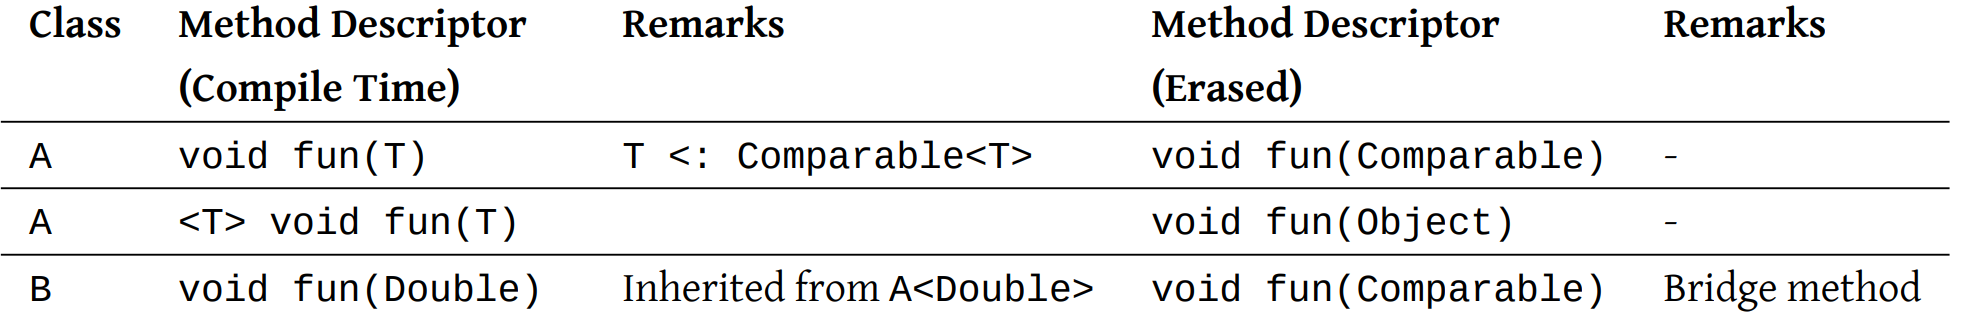
\includegraphics[width=1\linewidth]{Paper/Midterm/images/midterm-4.png}
            \item Build the method descriptor searching table \\
            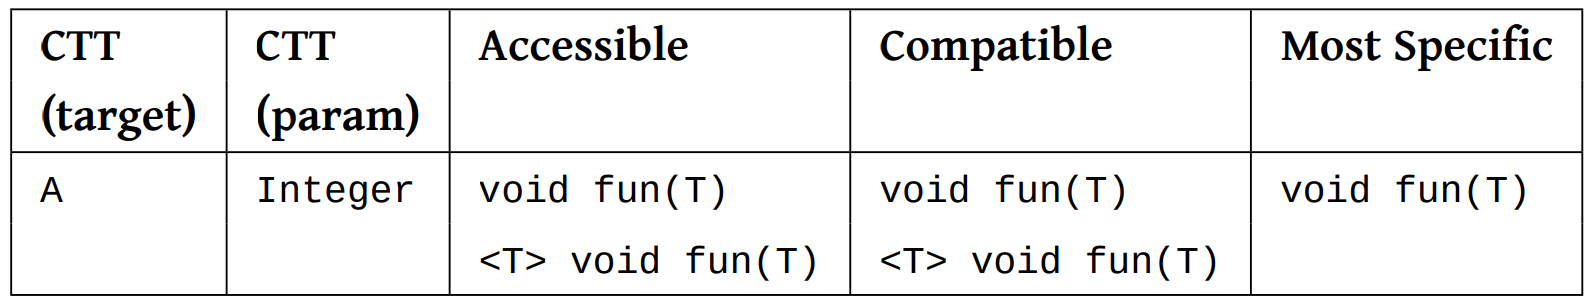
\includegraphics[width=1\linewidth]{Paper/Midterm/images/midterm-3.png} \\
            The accessible and compatible are the \textbf{method descriptors}, It is also recommended to add two columns, \textbf{erased method descriptor} and the \textbf{method invocated}
        \end{itemize}
    \end{itemize}
    \item \textbf{Abstract class}: An abstract class in Java is a class that has been made into something so general that it \textbf{cannot be instantiated}! And it \textbf{can} have the following:
    \begin{itemize}
        \item \textbf{Abstract method}: An abstract method \textbf{should not have} any method body but it \textbf{may throw an exception}! An abstract class without an abstract method is also allowed!
        \item \textbf{Concrete method}: As the name suggests, methods that are \textbf{not} abstract are concrete!
        \item \textbf{Instance/Class Field}: fields with \texttt{static} or without.
    \end{itemize}
    \item \textbf{Concrete Class}:
    \begin{itemize}
        \item a concrete class must have \textbf{implementations for all inherited abstract methods} (if it extends an abstract class or implementst an interface). Otherwise, a \textbf{compile error}!
        \item Beyond that, it’s free to have whatever you want — or even nothing at all in terms of fields or methods.
    \end{itemize}
    \item \textbf{Interface}:
    \begin{itemize}
        \item Interface \textbf{cannot} have \textbf{fields} and \textbf{concrete methods}!
        \item If \texttt{C implements I}, then we have \textbf{C $<$: I}. \textbf{A class can implement multiple interfaces.}
        \item Given a class A and an interface I, even if we didn't specify \texttt{A implements I}, the code \texttt{I i = (I) new A();} still compiles because we are not sure \textbf{whether there is a subclass of A that implements I}. \textbf{If so, no compile and runtime error will be generated. If not, no compile error will be generated but a runtime error will be generated.}
        \item \textbf{Always pay attention to the subtype realtionship containing interface}.
    \end{itemize}
    \item \textbf{\texttt{Object::equals}}: It will compare whether two objects are referenced to the \textbf{same memory address} or not.
    \textbf{Note}: To override this function from \texttt{Object} so it behaves as we want, we need to 
    \begin{itemize}
        \item check the RTT of \texttt{obj} is a \textbf{subtype} of the type we are interested (can be generic type), by using \texttt{if (obj instanceOf TYPE)}, if the TYPE is a generic type, it \textbf{must be an unbounded generic type, e.g. \texttt{A<?>}, it cannot be \texttt{A<String>}}
        \item typecast \texttt{obj} to the type we are interested by using either the class name or generic type with unbounded wildcard, e.g. \texttt{Box<?>}, \textbf{always be careful when you want to type cast to a generic type, since you are casting it to a rawtype!}
        \item Always pay attention to whether the \texttt{Object::equals(Object)} \textbf{has been overridden or not}. \textbf{If not, it will always compare whether two instances are the same or not}!
    \end{itemize}
\end{enumerate}

\section{Exception \& Wrapper Class}
\begin{enumerate}
    \item \textbf{Wrapper class}
    \begin{itemize}
        \item \textbf{Auto-boxing}, e.g. \texttt{Integer i = 4}, only happens on \textbf{primitive type}. \textbf{Complex type}, like Java array, doesn't support auto-boxing. e.g. \texttt{int[]} won't be converted to \texttt{Integer[]} automatically.
        \item \textbf{Unboxing also happens automatically}, it converts an instance of a wrapper class to its primitive type.
        \item Wrapper class objects are \textbf{immutable}, meaning that once you instantiate, changing the value will result in creating a new instance.
    \end{itemize}
    \item \textbf{Variance Relationship}: Let \texttt{S} denote the type of element in the ``array''. Then the \textbf{complex type} have three possible variance relationship:
    \begin{itemize}
        \item \textbf{Covariant}: if \texttt{S <: T}, then \texttt{C(S)<:C(T)}. e.g.e \textbf{Java array \texttt{Integer[] <: Double[]}} \textbf{int[] $</:$ double[]}
        \item \textbf{Contravariant}: if \texttt{S <: T}, then \texttt{C(T) <: C(S)}
        \item \textbf{Invariant}: it is neither \textbf{covariant} nor \textbf{contravariant}.
    \end{itemize}
    \item \textbf{Application of CTT and RTT}
    \begin{itemize}
        \item (\textbf{CTT}): To see whether a code will generate compile-error or not, we only see the CTT of the variable and the \textbf{type casting}.
        \item (\textbf{RTT}): \textbf{Run-time} error judgment \textbf{only} needs us to see the \textbf{RTT} of the variable. We \textbf{must ignore} the type casting because Java is \textbf{strongly typed}, meaning objects always retain their actual type (RTT).
        \item \texttt{(C) new B()} means the CTT is first B and then explicitly casted to C.
    \end{itemize}
    \item \textbf{Exception}: \textbf{Exceptions always happen at runtime!}
    \begin{itemize}
        \item \textbf{Unchecked Exception}: It is a subclass of \texttt{RuntimeException}, which is a subclass of \texttt{Exception}. \textbf{Not necessary to be handled} but it is recommended to do so. If not, \textbf{compile error} will be generated!
        \item \textbf{Checked Exception}: It is a subclass of \texttt{Exception}. \textbf{Must be handled}. 
        \item \textbf{Handle the exception}:
        \begin{itemize}
            \item This \textbf{must be done} in the \texttt{\textbf{catch}} block or be passed to another ``catch'' block. If there is no need for the \texttt{finally} block, can omit it.
            \item In the catch block, if there are blocks that are \textbf{unreachable}, a \textbf{compile error will be generated}!
        \end{itemize}
        \item If we have the code \texttt{int[] arr = new int[3]; arr[5]=10}, it \textbf{won't generate compile error, but will generate runtime error}!
        \item When an inner function throws a \textbf{checked exception}, if its outer function didn't handle it, it will ``pass'' the exception all the way until it is caught (\textbf{throw} immediately).
        \item The \texttt{finally} block is \textbf{always executed} even when \texttt{return} or \texttt{throw} is called in a \texttt{catch} block. (\texttt{throw} can be interpreted as \texttt{return} for easy understanding)
        \item It is possible for an Overriden method to throw the \textbf{same exception} or \textbf{any of its subtypes} as the method in the\textbf{ parent class}. \textbf{Throwing a supertype of the parent class's exception is not allowed}!
    \end{itemize}
\end{enumerate}

\section{Generics \& Wildcards}
\begin{enumerate}
    \item \textbf{Generic Type}:
    \begin{itemize}
        \item \textbf{Constructor}: the constructor of a generic type shouldn't contain \texttt{<>} operator. \textbf{Note}: when we \textbf{call} the constructor, we \textbf{must include \texttt{<>} operator}
        \item \textbf{Factory method}: it is a \textbf{class} method (declared with \texttt{static}) and a \textbf{generic} method (declare a method-level type parameter). e.g., \texttt{public static <T> Box<T> of(T obj) \{ return new Box<T>(obj); \}}. \textbf{Factory method is not a constructor!}
        \item \textbf{Parameterize a generic type}:
        \begin{itemize}
            \item When we use \texttt{extends} or \texttt{implements} a generic type \texttt{T}, we \textbf{must} instantiate the generic type \texttt{T}!
            \item When we call a method from a generic type, we should also \textbf{parameterize} the generic type either explicitly, e.g. \texttt{Box<String>}, or implicitly, e.g. \texttt{Box<>} (\textbf{must include \texttt{<>}})
            \item \textbf{Rule of Thumb}: Always think about \textbf{which generic type is the one you want to instantiate}!
        \end{itemize}
        \item \textbf{Subtype between generic type}: If you explicitly use \texttt{extends/implements}, e.g. \texttt{class A<T> extends B<T>}, then \texttt{A<T>} is a \textbf{subtype} of \texttt{B<T>}.
        \item \textbf{Bounded generic type parameter}: \texttt{T extends Class \& Interface}, \textbf{the first bound must be a class}! Otherwise, compile error will be generated!
        \item \textbf{Generics are invariant}: If \texttt{S<:T}, \textbf{\texttt{A<S> </:A<T>}}!
    \end{itemize}
    \item \textbf{Generic method}:
    \begin{itemize}
        \item \textbf{Method-Level Type parameter}: When a method declares its own generic type parameter with the \textbf{same name} as the class-level type parameter, the method-level type parameter will \textbf{shadow} the class-level type parameter within the method's scope. And \textbf{these two parameters are not the same}!
        \item \textbf{Class-level type parameter cannot be used in static method or static field}!
        \item \textbf{Non-static Generic method}: e.g. \texttt{public <U> Box<U> map \{\}, public Box<S> map \{\}}, this kind of method \textbf{may or may not} declare \textbf{method-level} type parameter, it can use \textbf{class-level} type parameter. And it depends on design requirements.
        \begin{itemize}
            \item \textbf{Invoke}: To invoke, we can use \texttt{instance.method()}
            \item \textbf{Non-static generic method cannot be parameterized using \texttt{<>}}! Otherwise, a \textbf{compile error} will be generated!
        \end{itemize}
        \item \textbf{Static Generic method}: e.g. \texttt{public static <T> Box<T> ofNullable(T obj) \{ \}}, this kind of method \textbf{must be declared using a method-level type parameter}.
        \begin{itemize}
            \item \textbf{Invoke}: To invoke, we can use \texttt{ClassName.<Type>method()}, or we can \textbf{omit} the \texttt{<Type>} to let the compiler do the type inference.
        \end{itemize}
        \item \textbf{Field-level type parameter}: Java \textbf{doesn't have} field-level type parameter!
    \end{itemize}
    \item \textbf{Type erasure}
    \begin{itemize}
        \item Replace \textbf{generic type} with its \textbf{raw type}.
        \item Replace type parameters.
        \begin{itemize}
            \item \textbf{Non-bounded type parameters} are replaced with \texttt{Object}
            \item \textbf{Bounded type parameters} are replaced with \textbf{the first bound} and \textbf{explicitly cast to the second bound}.
        \end{itemize}
        \item Insert necessary cast (Usually narrowing conversion) to make sure casting to the expected type.
        \item \textbf{Example}: this code \texttt{<U extends Container> void check(U con) \{\}} will become \texttt{void check(Container con) \{\}} \textbf{after type erasure}.
    \end{itemize}
    \item \textbf{Raw Type}
    \begin{itemize}
        \item The \textbf{Type erasure} of the raw type doesn't have the last \textbf{casting step}. The remaining is the same.
        \item When you use \textbf{raw type} in your code, there will always be a \textbf{rawtype warning}. (\textbf{Note that using unbounded wildcard \texttt{<?>} to replace rawtype won't generate a rawytype warning!}
        \item If rawtype is used, inside the generic type, all the type parameter will become \texttt{Object} or the \textbf{first bound}! Remember this!
        \item \textbf{Classic Example} \\
        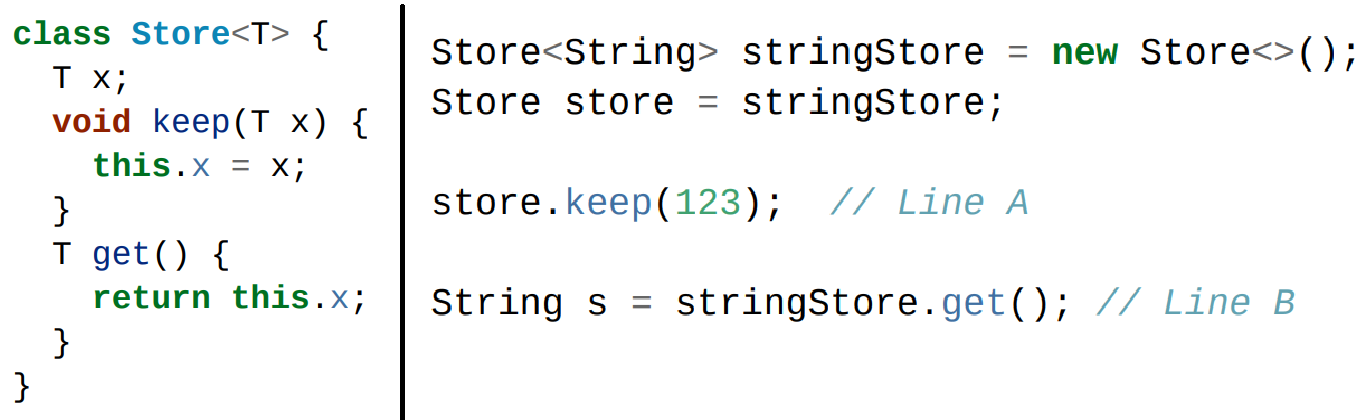
\includegraphics[width=1\linewidth]{Paper/Midterm/images/midterm-5.png} \\
        During compile time, \texttt{T} in \texttt{store} is \texttt{Object}, thus \texttt{Integer} is allowed!. During run-time, type erasure erased all \texttt{T} to \texttt{Object}. Thus, Line A is also allowed, but since Line B involves explicit casting between \texttt{String} and \texttt{Object}, this is not allowed!
    \end{itemize}
    \item \textbf{Generic Array}:
    \begin{itemize}
        \item We \textbf{cannot instantiate} a Java array using the type parameter, e.g. \texttt{new T[]} is not allowed. However, we \textbf{can declare} a Java array using the type parameter, e.g. \texttt{T[]} a is allowed.
        \item \textbf{An example}: \texttt{@SuppressWarnings("unchecked")}, then \texttt{Queue<Passenger>[] temp = (Queue<Passenger>[]) new Queue<?>[totalStops]}
        \item The generic array you declared after using the above method is \textbf{nothing but a Java Array}, it has \texttt{length} property!
    \end{itemize}
    \item \textbf{Bridge method}: A bridge method is \textbf{always generated} when, 1) a type \textbf{extends/implements a parameterized type} and 2)type erasure\textbf{ changes the signature} of \textbf{one or more inherited method}, which makes direct overriding impossible. \\
    \centerline{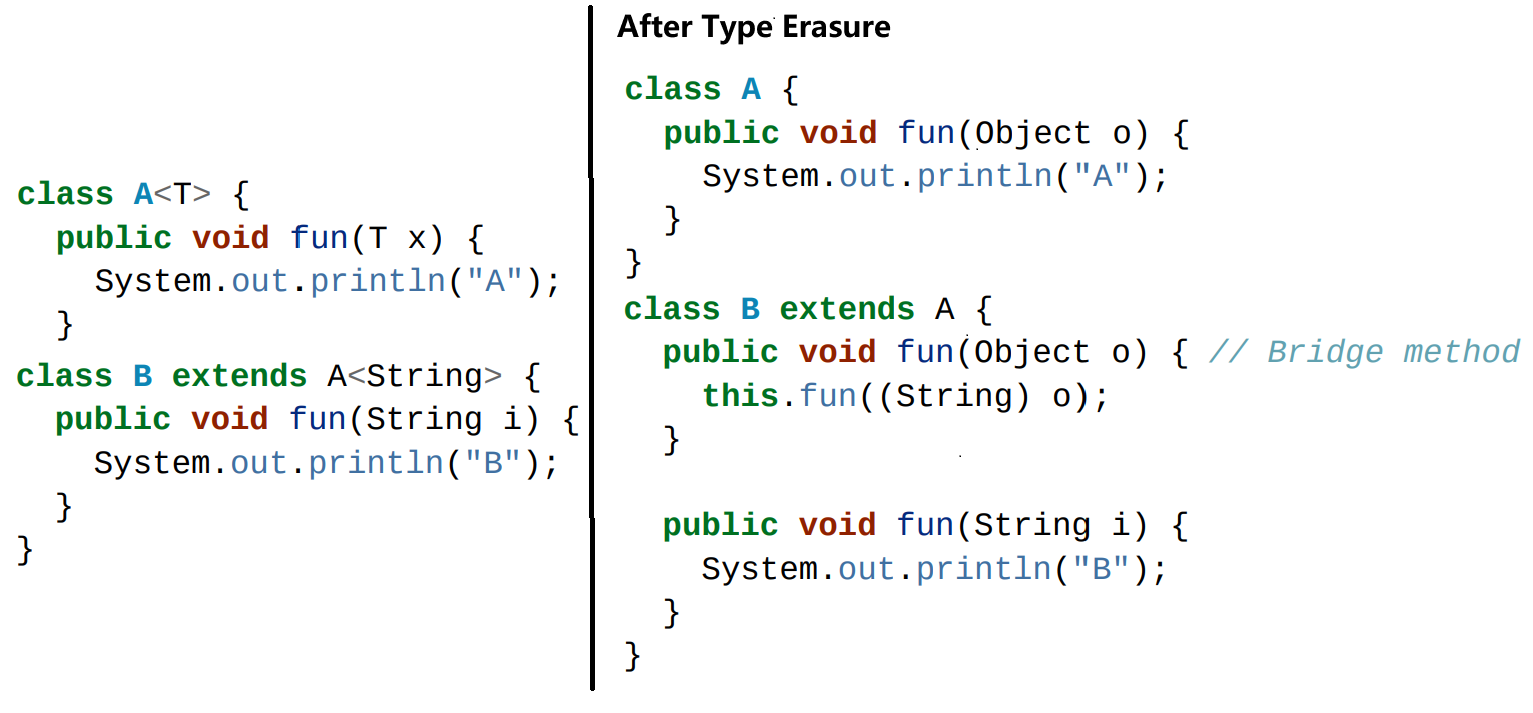
\includegraphics[width=1\linewidth]{Paper/Midterm/images/midterm-2.png}}
    \begin{itemize}
        \item \textbf{Steps}:
        \begin{itemize}
            \item copy the erased method into the subclass.
            \item Insert the cast using the \textbf{type argument} and call the available method using \texttt{this} (If \textbf{can} find a method matching the argument type, a.k.a subclass overrides the superclass) or \texttt{super} (If \textbf{cannot} find such a method, a.k.a no overriding).
        \end{itemize}
        \item \textbf{Calling bridge method}: With the above example, the following code will call the bridge method \texttt{A<String> a = new B(); a.fun("2");} and it will print ``B''. Notice when you use \texttt{A<String>}, the type parameter in class A will be \textbf{indicated} as \texttt{String}, treat \texttt{T} as \texttt{String} when \textbf{finding the method descriptor}, but when storing the method descriptor, still treat it as \texttt{Object}.
        \item Bridge methods only appear when overriding a \textbf{method} that uses the \textbf{class’s type parameter}.
    \end{itemize}
    \item \textbf{PECS Rule}: Producer \texttt{extends}, consumer \texttt{super}. \textbf{Note that PECS is usually used on method parameter.} An easy way to think of it is as follows
    \begin{itemize}
        \item Take the method parameter as your \texttt{studyObject}
        \item look at the \texttt{studyObject.method()}
        \item If \texttt{.method()} is something like \texttt{get(), read()}, then your \texttt{studyObject} is a producer, add \textbf{lower-bounded wildcard} to your method parameter.
        \item If \texttt{.method()} is something like \texttt{set(), write()}, then your \texttt{studyObject} is a consumer, add \textbf{upper-bounded wildcard} to your method parameter.
    \end{itemize}
    \item \textbf{Wildcards}
    \begin{itemize}
        \item Wildcards \textbf{is not a type!}, so, you \textbf{cannot} use them in class declaration and \textbf{cannot use them as type arguments}! But wildcards \textbf{can be used to instantiate an array of generic types}.
        \item \textbf{The following is not allowed}
        \begin{itemize}
            \item \texttt{private static final Box<?> emptyBox = new Box<?>(null);}
            \item \texttt{public <T> of(<? extends T>[], int depth) {}}
        \end{itemize}
        \item \textbf{Upper-Bounded Wildcards}: A\textless? extends T\textgreater, an upper-bounded wildcard allows a generic type to accept any \textbf{subtype} of a specified class or interface \texttt{T}. 
        \begin{itemize}
            \item If \texttt{S<:T}, then A\textless? extends S\textgreater \textless: A\textless? extends T\textgreater \textbf{(Covariance)} It will be beneficial to use \textbf{subtype is nothing but subset} to understand this relationship!
            \item For any type \texttt{S}, A\textless S\textgreater \textless: A\textless? extends S\textgreater
        \end{itemize}
        \item \textbf{Lower-Bounded Wildcards}: A\textless? super T\textgreater, a lower-bounded wildcard allows a generic type to accept any \textbf{supertype} of a specified class or interface \texttt{T}.
        \begin{itemize}
            \item If \texttt{S<:T}, then A\textless? super T\textgreater\textless:A\textless? super S\textgreater \textbf{(Contravariance)}.
            \item For any type \texttt{S}, A$<$S$>$ $<$: A$<$? super S$>$
        \end{itemize}
        \item \textbf{Unbounded Wildcards}: \texttt{A<?>}
        \begin{itemize}
            \item \texttt{A<?>} is the \textbf{supertype} of every \textbf{parameterized type} of \texttt{A<T>}, that is \texttt{A<T><:A<?>}.
        \end{itemize}
        \item During \textbf{Type erasure}, wildcards will be erased! And generics become the \textbf{raw type}!
    \end{itemize}
    \item \textbf{Type inference}
    \begin{itemize}
        \item \textbf{Rule to find constraints}
        \begin{itemize}
            \item \textbf{Target}: ``the \textbf{return type} of the method'' <: ``the type of the variable you are assigning to''
            \item \textbf{Argument}: ``the type of the \textbf{argument}'' <: ``the type of the \textbf{parameter}''
            \item \textbf{Bound}: we need to consider ``the \textbf{bound of the generic type parameters}''
        \end{itemize}
        \item \textbf{Rules to solve constraints}
        \begin{itemize}
            \item \texttt{Type1<:T<:Type2}, then \texttt{T} is inferred as \texttt{Type1}
            \item \texttt{Type1<:T}, then \texttt{T} is inferred as \texttt{Type1}
            \item \texttt{T<:Type2}, then \texttt{T} is inferred as \texttt{Type2}
        \end{itemize}
        \item \textbf{Type inference involves wildcard}
        \begin{itemize}
            \item If parameter type is \texttt{Seq<? super T>}, argument type is \texttt{Seq<G>}, then \texttt{T<:G}
            \item If parameter type is \texttt{Seq<? extends T>}, argument type is \texttt{Seq<G>}, then \texttt{G<:T}
        \end{itemize}
        \item If \texttt{class A implements Comparable<A>}, and \texttt{class B extends A}, then \texttt{B} actually implements \texttt{Comparable<A>} \textbf{not} \texttt{Comparable<B>}!
    \end{itemize}
\end{enumerate}

\end{multicols}

\end{document}